%% open-cam: IS&T Electronic Imaging 2027 proceedings paper.
%% Build: see README.md (latexmk -pdf open_cam_ei2027.tex).
\documentclass[letterpaper,twocolumn,fleqn]{article}
\usepackage{ist}
\usepackage{microtype}
\usepackage{booktabs}
\usepackage{graphicx}
\usepackage{amsmath}
\usepackage{url}
\usepackage[hidelinks]{hyperref}
\emergencystretch=1.5em

%% Numbers produced by scripts/fig_mtf.py (figures/mtf_summary.json).
\newcommand{\mtfFoc}{0.209}
\newcommand{\mtfDefTwo}{0.270}
\newcommand{\mtfDefFive}{0.294}
\newcommand{\mtfNyqFoc}{0.127}
\newcommand{\mtfLamBest}{423}
\newcommand{\mtfLamRange}{0.201--0.221}

\title{open-cam: an open-source hyperspectral, ray-traced camera simulator built on pbrt-v4 for sensor, lens and CFA studies}

\author{Brian Deegan;
        University of Galway;
        Galway, Ireland}

\date{}

\begin{document}
\maketitle
\thispagestyle{empty}

\begin{abstract}
We present open-cam, an open-source (MIT) camera simulator that couples the physically based renderer pbrt-v4 with a radiometrically explicit sensor model. Unlike most driving and robotics simulators, open-cam never forms an RGB image inside the renderer: pbrt-v4 writes per-wavelength radiance buckets, which are converted to sensor-plane irradiance, photon counts and photoelectrons with measured quantum efficiency and infrared-cut-filter curves, then passed through an EMVA1288-style noise, ADC and colour filter array model. Lenses can be traced through real prescriptions. We describe the architecture, compare it with open-source and commercial camera simulators, and report reproducible validation: an end-to-end ColorChecker render, a photon-transfer check that recovers the configured system gain to within 0.3\%, a traced-lens slanted-edge MTF, and a study of non-Bayer filter arrays derived from a single spectral render. We are explicit about current limitations, notably that only Bayer mosaics are sampled and demosaiced end-to-end.
\end{abstract}

\section{Introduction}
Camera simulation is used to prototype sensors, to evaluate image signal processors (ISPs) and to generate training and test data for perception. Two families of tools exist. Image-systems simulators such as ISETCam~\cite{farrell2003simulation,farrell2012digital,isetcam} model the physics of light, optics and sensors in spectral units, while driving and robotics simulators (CARLA~\cite{dosovitskiy2017carla}, AirSim~\cite{shah2017airsim}, NVIDIA Isaac Sim~\cite{isaaccamera} and commercial platforms) emphasise real-time scene dynamics and typically render RGB images to which camera effects are added afterwards.

Many questions that matter in automotive and mobile imaging cannot be answered from an RGB render: how a red--clear--clear--blue (RCCB) or red--yellow--yellow--cyan (RYYCy) mosaic changes low-light signal-to-noise ratio (SNR), how the infrared-cut filter (IRCF) interacts with an LED or tungsten illuminant, or how a lens with longitudinal chromatic aberration blurs each colour channel. All require the spectral radiance at the sensor. open-cam~\cite{opencam} is a Python toolkit built to answer such questions with free tools. Its contributions are: (i) a spectral pipeline from pbrt-v4~\cite{pharr2023pbrt,pbrtv4code} spectral film to photoelectrons, with every radiometric factor explicit; (ii) an EMVA1288-style~\cite{emva1288std} sensor model with analytic validators and real-renderer end-to-end tests; (iii) a library of camera recipes, measured spectral data and traced lens prescriptions; and (iv) an honest account of what is and is not yet implemented, in particular for non-Bayer colour filter arrays (CFAs).

\section{Related work}
\textbf{Image-systems simulation.} ISETCam (MATLAB, MIT licence) keeps scene spectral radiance, optical-image irradiance and sensor photoelectrons and voltages in physical units, and includes models of CFAs, optics and displays~\cite{isetcam,farrell2012digital}. ISET3D (MIT) adds 3D rendering with pbrt-v4~\cite{iset3d}; it has been validated against measured cameras~\cite{lyu2021cornell,lyu2022validation} and extended with ray-transfer functions for lenses whose design is hidden~\cite{goossens2022ray}. ISETAuto (Apache-2.0) applies the stack to driving scenes and network evaluation~\cite{isetauto,blasinski2018optimizing,liu2019soft}. open-cam is closest to this family; it differs in being pure Python, in its configuration-driven catalogue of 73 camera recipes, and in its EMVA1288-oriented validators and continuous-integration tests that run the real renderer. It does not yet offer the breadth of ISETCam's optics, display and human-vision models.

\textbf{Renderers.} pbrt-v4 (Apache-2.0) renders with spectral sampling and provides a \texttt{spectral} film that stores radiance in wavelength buckets, as well as a \texttt{realistic} camera that traces a lens prescription~\cite{pharr2023pbrt,pbrtv4format,kolb1995realistic}. Mitsuba~3 (BSD-style licence) offers spectral and polarised variants~\cite{nimier2019mitsuba2,mitsuba3variants}. Both are renderers, not camera models: they stop at radiance or at a colour image.

\textbf{Driving and robotics simulators.} CARLA (MIT) renders RGB cameras with Unreal Engine post-processing; its documented camera attributes include auto exposure, bloom, grain jitter and lens-distortion parameters~\cite{carlasensors}. AirSim (MIT) exposes noise and distortion settings for its RGB cameras~\cite{airsimsettings}; Gazebo models camera noise as independent Gaussian noise per pixel~\cite{gazebonoise}. NVIDIA Isaac Sim's RTX camera documents OpenCV pinhole and fisheye distortion models, additive noise, encoding of the RGB image into a single-channel Bayer mosaic and an on-chip ISP stage~\cite{isaaccamera}; NVIDIA's DRIVE simulation stack advertises high-fidelity sensor simulation~\cite{nvidiadrivesim}. None of these documentations describe spectral rendering into a QE-weighted sensor.

\textbf{Commercial sensor and optics tools.} Ansys Speos performs spectral, wavelength-dependent ray tracing with camera and detector response simulation~\cite{ansysspeos,falahati2026speos}; Ansys AVxcelerate Sensors provides a real-time, physics-based camera model parameterised from a camera datasheet and a multispectral material database~\cite{ansysavx}. Lens-design packages (Ansys Zemax OpticStudio~\cite{ansyszemax}, Synopsys LightTools~\cite{synopsyslighttools}) provide sequential and non-sequential ray tracing and stray-light analysis. Scenario-level platforms, including Siemens Simcenter Prescan~\cite{siemensprescan}, IPG CarMaker~\cite{ipgcarmaker}, Hexagon VTD~\cite{son2023vtd}, rFpro~\cite{rfproraytracing}, Cognata~\cite{cognata} and dSPACE AURELION, describe ``physics-based'' or ray-traced sensor simulation; rFpro, for example, documents a multi-exposure HDR camera API with motion blur~\cite{rfproraytracing}. Foretellix~\cite{foretellix} targets scenario generation and coverage rather than sensor physics. For these commercial tools the spectral resolution, noise model and CFA options are not specified in the public material we could access, so Table~\ref{tab:compare} marks them as not publicly documented rather than guessing. Pricing is quote-based throughout.

\textbf{Measurement.} EMVA1288~\cite{emva1288std,borek2023emva}, photon transfer~\cite{janesick2007photon} and ISO~12233 slanted-edge analysis~\cite{iso12233,williams2003lowfreq} define how real cameras are characterised; the EMVA1288 reference implementation (LGPL-3.0)~\cite{emva1288py} and commercial suites such as Imatest~\cite{imatest} implement them for measured data. open-cam uses the same definitions so that simulated and measured cameras can be compared on equal terms.

\begin{table*}[t]
\caption{Camera-simulation capabilities as stated in each tool's public documentation or papers (accessed October 2026). ``n.d.'' = not documented in the public sources we reviewed; it does not mean the capability is absent.}
\label{tab:compare}
\vspace{14pt}
\centering\small
\begin{tabular}{@{}p{2.5cm}p{2.5cm}p{2.4cm}p{3.0cm}p{2.9cm}p{2.3cm}@{}}
\toprule
Tool & Spectral rendering & Ray-traced lens & Sensor noise / EMVA1288 & CFA flexibility & Licence / cost \\
\midrule
open-cam & Yes: pbrt-v4 spectral film, user-set buckets & Yes: pbrt-v4 realistic camera, 4 prescriptions & Shot, read, PRNU, DSNU, dark current, ADC, FPN, defects; EMVA validators & Arbitrary QE curves; Bayer (4 phases) end-to-end only & MIT; free \\
ISETCam / ISET3D / ISETAuto & Yes (spectral radiance) & Yes (pbrt-v4; ray-transfer functions) & Physical photoelectron/voltage model & CFA models included~\cite{isetcam} & MIT / Apache-2.0; MATLAB required \\
pbrt-v4, Mitsuba 3 & Yes & pbrt-v4: realistic camera & None (renderer) & None & Apache-2.0 / BSD; free \\
CARLA, AirSim, Gazebo & No (RGB) & No; distortion parameters & Grain / Gaussian / noise-line effects & None (RGB output) & MIT / Apache-2.0; free \\
Isaac Sim (RTX) & n.d. & No; OpenCV distortion models & Additive noise & Bayer encoding + ISP & NVIDIA licence \\
Ansys Speos & Yes & Yes & Detector response, raw signal & n.d. & Commercial \\
Ansys AVxcelerate & Multispectral materials & n.d. & Datasheet-parameterised & n.d. & Commercial \\
Zemax OpticStudio, LightTools & Wavelength-dependent tracing & Yes (lens design) & n.d. & n.d. & Commercial \\
Prescan, CarMaker, VTD, rFpro, Cognata, AURELION, DRIVE Sim & n.d. & n.d. (rFpro: ray tracing) & n.d. & n.d. & Commercial \\
Imatest, emva1288 & -- (measurement) & -- & EMVA1288 analysis of measured data & -- & Commercial / LGPL-3.0 \\
\bottomrule
\end{tabular}
\end{table*}

\section{Architecture}
open-cam is a set of command-line tools orchestrated by \texttt{tools/run\_pipeline.py}. A single YAML file (\texttt{config/pipeline.yaml}) selects a camera recipe and drives four stages: scene generation, pbrt-v4 rendering, spectral-to-electron conversion and the sensor/noise/CFA stage, followed by validators. A recipe in \texttt{config/camera\_recipes/} (73 are provided: phone, compact, interchangeable-lens and research cameras) references a sensor model (QE curves, pixel pitch, fill factor, exposure, EMVA parameters, CFA) and a lens model. Sensor models are written as deltas from \texttt{config/sensor\_models/default.yaml}, so a new sensor needs only its overrides.

\textbf{Scenes.} \texttt{build\_colorchecker\_scene.py} builds a 24-patch ColorChecker from measured X-Rite reflectances lit by a tabulated illuminant (D50--D75, A, C, fluorescent and LED spectra are included). \texttt{build\_image\_quality\_targets.py} generates slanted-edge, Siemens-star and ISO-style noise targets, and \texttt{build\_munsell\_scenes.py} builds charts from 1269 measured Munsell chips (380--800\,nm at 1\,nm).

\textbf{Spectral rendering.} Scenes are rendered with pbrt-v4's \texttt{spectral} film, which writes an OpenEXR file with one radiance channel per wavelength bucket (\texttt{S0.<}$\lambda$\texttt{>nm}, in W\,m$^{-2}$\,sr$^{-1}$\,nm$^{-1}$)~\cite{pbrtv4format}. The default pipeline uses 64 buckets between 360 and 830\,nm. Cameras can be pinhole, thin-lens or pbrt-v4's \texttt{realistic} camera, which traces rays through a lens prescription~\cite{kolb1995realistic}. The repository ships four prescriptions (a 22\,mm wide-angle, a 50\,mm double-Gauss, a 250\,mm telephoto and a 10\,mm fisheye) and 14 lens models that bind them, or thin-lens parameters, to camera classes.

\textbf{Radiance to electrons.} Radiance is converted to sensor-plane irradiance by \texttt{pbrt\_spectral\_exr\_to\_electrons.py} using the camera equation
\begin{equation}
E_\lambda(x,y) = L_\lambda(x,y)\,\frac{\pi\,\tau(\lambda)}{4N^2(1+m)^2}\,c_{\mathrm{cal}},
\end{equation}
where $N$ is the f-number (taken from the traced prescription when the realistic camera is used), $m$ the magnification, $\tau$ the optics transmittance and $c_{\mathrm{cal}}$ an optional photometric calibration to a target scene illuminance. The mean electrons in channel $c$ are then
\begin{equation}
\mu_{e,c} = \sum_\lambda E_\lambda \frac{\lambda}{hc}\, \eta_c(\lambda)\, T_{\mathrm{IR}}(\lambda)\, \Delta\lambda\; A_{\mathrm{px}}\, t\, F\, V_c(x,y),
\end{equation}
with QE $\eta_c$, IRCF transmittance $T_{\mathrm{IR}}$, bucket width $\Delta\lambda$, pixel area $A_{\mathrm{px}}$, exposure time $t$, fill factor $F$ and an optional vignetting map $V_c$. The photon conversion, QE, bin widths and geometry are folded into a $K\times C$ weight matrix (\texttt{sensor\_radiometry.spectral\_electron\_weights}), so integration is a single matrix product per pixel. The same helper is shared with \texttt{spectral\_sensor\_forward.py}, an analytic forward model used for fast tests. QE curves for many cameras are taken from a measured spectral-sensitivity database; generic red, green, blue, cyan, yellow, magenta and monochrome curves and an IRCF are also provided.

\textbf{Sensor model.} \texttt{apply\_emva\_noise.py} implements the EMVA1288 linear camera model~\cite{emva1288std}: Poisson shot noise on signal plus dark current (with a temperature model), PRNU as a multiplicative gain map, DSNU as an additive offset map, Gaussian read noise, optional kTC noise, row/column fixed-pattern and flicker noise, hot/stuck pixels, blooming, inter-pixel crosstalk, full-well clipping and an ADC with gain $K$ (e$^-$/DN), black level, bit depth and optional INL/DNL. Spatial maps use a fixed seed (one ``camera unit'') while temporal noise uses a per-frame seed. A Bayer mosaic is sampled with any of the four RGGB/BGGR/GRBG/GBRG phases and demosaiced bilinearly or with the Malvar--He--Cutler algorithm~\cite{malvar2004high}. \texttt{apply\_spectral\_psf.py} adds post-render optics where a traced lens is not used: Gaussian, wavelength-dependent Gaussian and Airy-disk PSFs per spectral bucket, lateral chromatic aberration and stray light.

\textbf{Validation and tests.} \texttt{validate\_emva\_model.py} compares the analytic EMVA mean and variance with Monte Carlo at photon-transfer levels and checks the recipe against its datasheet block; \texttt{batch\_validate\_emva.py} runs this across all recipes. \texttt{validate\_demosaic\_linear.py} checks demosaic fidelity in linear DN. Twenty test modules include two that call the real pbrt-v4 binary: \texttt{test\_pbrt\_e2e.py} and \texttt{test\_pbrt\_full\_pipeline.py}. The latter renders a 96$\times$64, 16-bucket ColorChecker and, for every pixel, forms the residual
$z = (\mathrm{DN}-(b+\mu_e/K))/\sigma_{\mathrm{pred}}$ against the analytic EMVA prediction, requiring zero mean and unit variance; it also checks ADC limits, seed determinism and demosaic error.

\textbf{Teaching.} A Dear PyGui~\cite{dearpygui} desktop application (\texttt{gui/}) exposes the same engines through interactive scenarios on optics, PSF and aberrations, MTF, sensor noise, exposure and defects, colour/ISP and image generation, with accompanying tutorials.

\section{Results}
All results below were produced on a CPU build of pbrt-v4 with the scripts in \texttt{paper/ei2027/scripts/}; the exact commands are listed in the accompanying README. Renders are 960$\times$640.

\textbf{End-to-end ColorChecker.} We rendered the ColorChecker with the geometry and lens of \texttt{config/pipeline.yaml} (realistic 22\,mm wide-angle prescription, 8.756\,mm aperture, focus 4\,m, 1024 samples per pixel, 64 buckets over 360--830\,nm) under CIE D65 and CIE A, and ran it through the \texttt{iphone\_8} recipe (1.4\,\textmu m pixels, GBRG, Malvar demosaic, $K=9.906$\,e$^-$/DN, 9500\,e$^-$ full well, 10-bit) at 500\,lux and 0.12\,s, the pipeline defaults. With the realistic camera the effective f-number from the prescription is f/2.51. The white patch yields 364/821/439\,e$^-$ (R/G/B) under D65. Fig.~\ref{fig:cc} shows the demosaiced output with grey-world preview white balance; the gains change from 2.19/1.00/1.83 (D65) to 1.27/1.00/3.21 (A), a direct consequence of integrating each illuminant's spectrum against the camera QE rather than of an RGB tint. Against a noise-free reference, \texttt{validate\_demosaic\_linear.py} reports a Malvar demosaic error of 0.114\,DN MAE and 0.389\,DN RMSE.

\begin{figure*}[t]
\centering
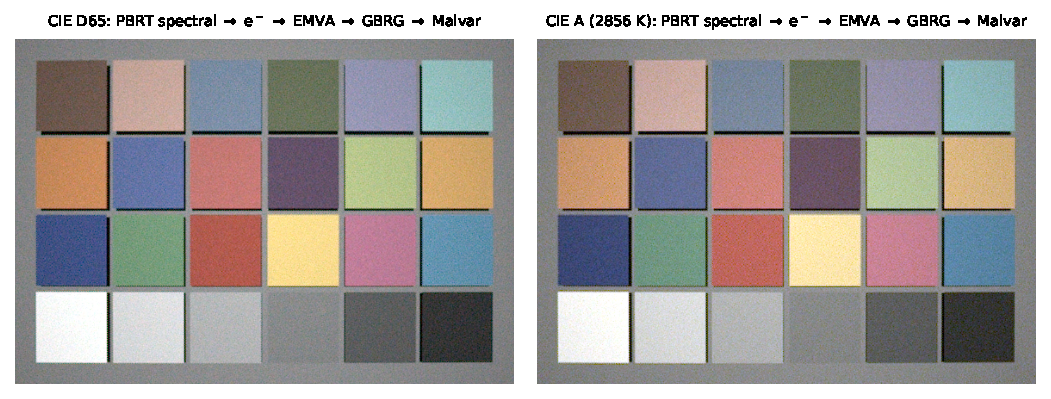
\includegraphics[width=\textwidth]{figures/fig_colorchecker.pdf}
\caption{ColorChecker rendered spectrally by pbrt-v4 (64 buckets) and processed by open-cam with the iphone\_8 recipe: electrons $\rightarrow$ EMVA noise $\rightarrow$ GBRG mosaic $\rightarrow$ Malvar demosaic, grey-world preview white balance, no colour correction. Left: D65; right: CIE A.}
\label{fig:cc}
\end{figure*}

\textbf{Photon transfer.} Using the iphone\_8 EMVA parameters ($\sigma_d=1.6$\,e$^-$, PRNU 1.8\%, DSNU 0.16\,e$^-$), we simulated 256$\times$256 uniform frame pairs at 29 exposure levels from dark to beyond saturation with \texttt{emva\_theory.simulate\_uniform\_stack}, and applied the EMVA1288 photon-transfer method (temporal variance from frame-pair differences; zero-intercept fit of $\sigma_y^2-\sigma_{y.\mathrm{dark}}^2$ against $\mu_y-\mu_{y.\mathrm{dark}}$ up to 70\% of full well). The fit recovers $K=9.883$\,e$^-$/DN against the configured 9.906 (0.23\% error) and $\sigma_d=1.588$\,e$^-$ (configured 1.6). The EMVA PRNU estimate from 16-frame dark and 50\%-saturation stacks is 1.79\% (configured 1.8\%). Across the linear range the simulated variance deviates from the analytic model by at most 1.3\% (median 0.46\%), consistent with the sampling error of a 65,536-pixel estimate (Fig.~\ref{fig:ptc}). \texttt{validate\_emva\_model.py} passes all photon-transfer, dark-frame and datasheet checks for this recipe with 20,000 Monte Carlo trials.

\begin{figure*}[t]
\centering
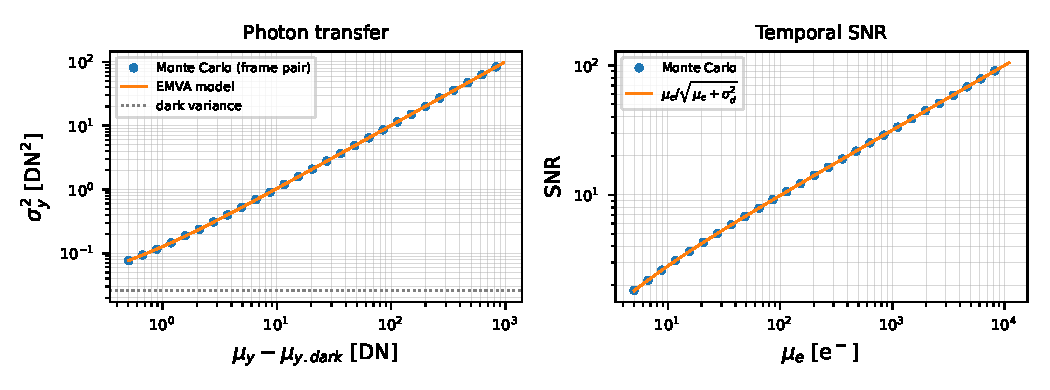
\includegraphics[width=0.85\textwidth]{figures/fig_ptc.pdf}
\caption{EMVA1288 photon-transfer validation for the iphone\_8 recipe. Left: temporal variance versus dark-subtracted mean signal for Monte Carlo frame pairs (markers) and the analytic model (line); the gain fit uses levels up to 70\% of full well. Right: temporal SNR versus mean electrons.}
\label{fig:ptc}
\end{figure*}

\textbf{Traced-lens MTF.} We rendered a 5$^\circ$ slanted edge at 3.2\,m through the 50\,mm double-Gauss prescription (32 buckets, 400--700\,nm) at f/2 in focus, at f/2 focused at 2.6\,m, and at f/5.6 focused at 2.6\,m, and analysed it with \texttt{sfr\_analysis.slanted\_edge\_sfr}. With the generic green QE the MTF50 is \mtfFoc, \mtfDefTwo{} and \mtfDefFive{}\,cy/px respectively, and the in-focus MTF at Nyquist is \mtfNyqFoc{} (Fig.~\ref{fig:mtf}). Two observations are worth reporting as measured rather than explained away. First, the nominal \texttt{focusdistance} of 3.2\,m is not the sharpest setting: focusing at 2.6\,m gives a higher MTF50, so a through-focus sweep, rather than the nominal value, should be used to find best focus with this prescription. Second, stopping down to f/5.6 raises MTF50 further, as expected from the smaller blur circle. Because the film is spectral, the same render also yields an MTF per wavelength bucket (Fig.~\ref{fig:mtf}, right). Here we report the data only with a caveat: the per-bucket MTF50 shows a periodic ripple of roughly $\pm$5\% with a period of about five buckets in all three renders, which is not plausible as a lens property and which we have not yet traced (pbrt-v4's stochastic wavelength sampling is a candidate). The bucket-to-bucket structure should therefore not be interpreted as chromatic aberration; resolving it, e.g.\ with monochromatic renders, is required before per-wavelength MTF can be used quantitatively. Edge positions were located with a 50\%-crossing fit after per-row flat-fielding, because the derivative-centroid estimator in \texttt{sfr\_analysis.py} was biased by render noise on this edge (it reported a $-2.3^\circ$ edge for a measured $-5.0^\circ$); the ESF binning, LSF and MTF use the repository functions. Note that these values are in film pixels of the renderer and include the pbrt-v4 Gaussian reconstruction filter.

\begin{figure*}[t]
\centering
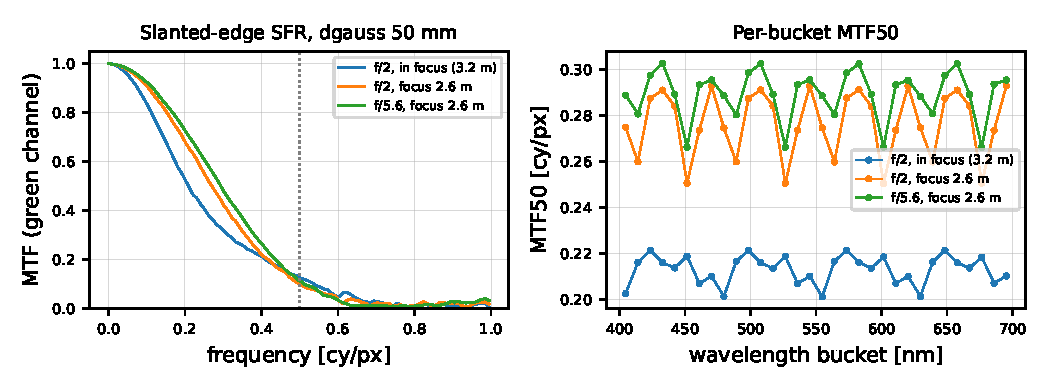
\includegraphics[width=0.85\textwidth]{figures/fig_mtf.pdf}
\caption{Slanted-edge MTF through the traced 50\,mm double-Gauss lens. Left: green-channel MTF for three aperture/focus settings (dotted line: Nyquist). Right: MTF50 computed separately in each spectral bucket of the same renders; the periodic ripple is unexplained (see text).}
\label{fig:mtf}
\end{figure*}

\textbf{CFA support: what exists.} We inspected the CFA path to state its scope precisely. \texttt{apply\_emva\_noise.py} samples and demosaics only 2$\times$2 Bayer phases and rejects other pattern names. The recipes named \texttt{default\_rccb}, \texttt{default\_ryycy}, \texttt{default\_rccg}, \texttt{default\_rggcy} and \texttt{default\_cmy} are \emph{RGB proxies}: the three QE slots of the Bayer path are filled with other curves (for RCCB, the ``clear'' channel is the generic cyan curve in the green slot; for RYYCy, yellow and cyan replace green and blue), and the result is still sampled on a Bayer lattice. RGBW, true clear pixels, quad-Bayer~\cite{okawa2019quad} and arbitrary $n\times n$ tiles are therefore not yet supported end-to-end, and there is no non-Bayer demosaicing.

\textbf{CFA support: what the spectral design enables.} Because the renderer output is spectral, any channel set can nonetheless be computed from the same EXR with the pipeline's own integration weights, and sampled on any tile. \texttt{fig\_cfa.py} does this outside the pipeline (no pipeline code is modified): it integrates the D65 and A ColorChecker renders against six QE$\times$IRCF curves (Fig.~\ref{fig:qe}), with ``W'' the unfiltered monochrome silicon QE, and anchors the absolute scale to the pipeline's green-channel electrons for the default recipe (the ratio is constant across all 24 patches to a coefficient of variation of $4\times10^{-8}$, confirming that the script and the pipeline implement the same radiometry). Fig.~\ref{fig:mosaic} shows raw mosaics for six layouts. Table~\ref{tab:cfa} reports, for the neutral 5 patch (about 19\% reflectance), the luminance-channel electrons at 500\,lux and the analytic EMVA temporal SNR, $\mu_e/\sqrt{\mu_e+\sigma_d^2}$ with $\sigma_d=2.6$\,e$^-$, scaled to 10\,lux. A clear pixel collects 2.62$\times$ the electrons of the green pixel and gains 6.0\,dB of SNR in this low-light case; yellow and the cyan proxy gain 2.8 and 3.2\,dB. These ratios depend on the illuminant: under CIE A the yellow/green ratio rises from 1.55 to 2.12 and the cyan/green ratio falls from 1.65 to 1.11. The spectral render also quantifies the error of the current RGB proxy: normalised on the white patch, the cyan-proxy/clear ratio ranges from 0.43 (patch 15, red) to 1.34 (patch 13, blue), so a cyan curve is not a scalar stand-in for a clear pixel, and the error depends on scene colour. Quad-Bayer has identical per-pixel statistics to Bayer here because binning and remosaicing are not modelled. Per-pixel analyses of this kind are impossible from an RGB render, which is why we regard the spectral representation, rather than the current CFA code, as open-cam's main asset for CFA research~\cite{hirakawa2008spatio}.

\begin{figure}[t]
\centering
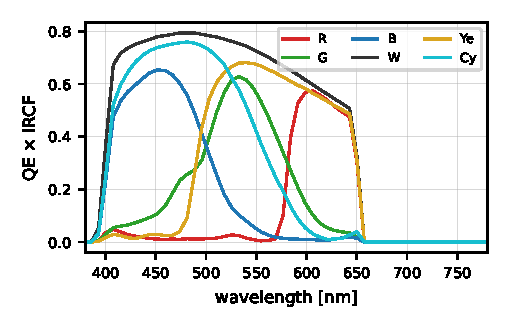
\includegraphics[width=\columnwidth]{figures/fig_qe.pdf}
\caption{Generic QE$\times$IRCF curves shipped in \texttt{spectra/QE/interpolated/} and used for the CFA study (W: unfiltered monochrome QE).}
\label{fig:qe}
\end{figure}

\begin{figure}[t]
\centering
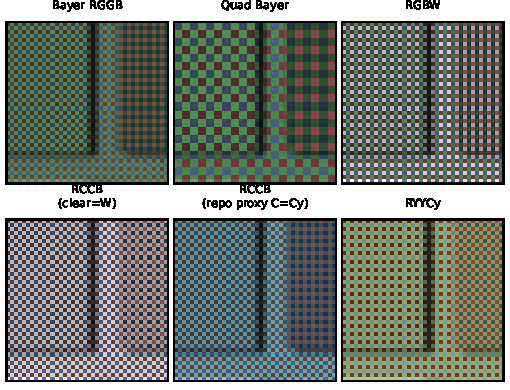
\includegraphics[width=\columnwidth]{figures/fig_cfa_mosaics.pdf}
\caption{Raw mosaics computed from one spectral render (D65) at the corner of patches 14, 15, 20 and 21, each pixel tinted by its filter. Only Bayer is sampled by the pipeline itself; the other layouts are produced by \texttt{fig\_cfa.py} from the same spectral buckets.}
\label{fig:mosaic}
\end{figure}

\begin{table}[t]
\caption{Luminance-channel signal on the neutral 5 patch from one D65 render (default recipe, 0.12\,s) and analytic temporal SNR at 10\,lux.}
\label{tab:cfa}
\vspace{14pt}
\centering\small
\begin{tabular}{@{}lcccc@{}}
\toprule
CFA (channel) & $\mu_e$ @500\,lx & SNR @10\,lx & $\Delta$ & ch/G (A) \\
\midrule
Bayer / quad (G) & 282 & 4.1\,dB & -- & 1.00 \\
RGBW, RCCB (W) & 741 & 10.1\,dB & +6.0\,dB & 2.67 \\
RCCB proxy (Cy) & 465 & 7.3\,dB & +3.2\,dB & 1.11 \\
RYYCy (Ye) & 438 & 6.9\,dB & +2.8\,dB & 2.12 \\
\bottomrule
\end{tabular}
\end{table}

\section{Discussion and limitations}
The results support the central design choice: keeping light spectral until the photon-counting step makes illuminant, IRCF and filter questions first-class, and the EMVA validators make the noise model auditable against datasheets. The limitations are equally concrete. Non-Bayer CFAs are not sampled or demosaiced in the pipeline; the natural extension is to generalise the Bayer lookup tables in \texttt{apply\_emva\_noise.py} to an $n\times n$ tile of named QE curves with per-tile demosaicing, which the spectral integration already supports. Many recipes carry EMVA parameters inferred from public tables (each recipe records a calibration tier) rather than measured reports. Rendering is offline: the 1024-sample, 64-bucket ColorChecker took roughly 4.5\,min on an 8-core CPU, so open-cam complements rather than replaces real-time simulators. Scenes are currently charts and targets rather than driving environments, and there is no motion blur, rolling shutter or HDR multi-exposure model yet.

\section{Conclusion}
open-cam provides a free, scriptable path from pbrt-v4 spectral radiance to EMVA-consistent raw data through traced lenses and measured QE curves. It recovers configured sensor parameters through the EMVA1288 photon-transfer method, reproduces illuminant-dependent white balance from first principles, and, while its pipeline CFA support is currently Bayer-only, its spectral representation already allows quantitative studies of RGBW, RCCB and RYYCy designs. Code, configurations and all scripts used for this paper are available at \url{https://github.com/briandeegan82/open-cam}.

\small
\bibliographystyle{ieeetr}
\bibliography{references}

\begin{biography}
Brian Deegan is with the University of Galway, Ireland. His research focuses on camera image quality, sensor and optics modelling, and simulation for automotive imaging.
\end{biography}

\end{document}
